\documentclass{article}
\usepackage[utf8]{inputenc}
\usepackage{graphicx}
\usepackage{hyperref}
\setlength{\oddsidemargin}{0in}
\setlength{\evensidemargin}{0in}
\setlength{\textheight}{9in}
\setlength{\textwidth}{6.5in}
\setlength{\topmargin}{-0.5in}

\title{122B Spring 2016 \\ Program 2}
\author{Russell Miller and Rylan Schaeffer }
\date{June 2016}

\begin{document}

\maketitle

\section*{Introduction}
\indent \indent Quicksort, Quickselect and Deterministicselect are three algorithms that can be used to select the $k$th smallest element of an unordered list. We sought to compare their performance (measured by time to correct result) as a function of list length. To do so, we performed an analysis of the algorithms and gathered experimental data from randomly generated lists to confirm our analysis. We conclude that although the three algorithms' performances are comparable for short lists, the performances begin to differ for longer lists, with quicksort emerging as the clear winner.

\section*{Analysis of Algorithms}
\subsection*{Quickselect}
\indent \indent 

\subsection*{Deterministicselect}
\indent \indent 

\subsection*{Quicksort with Select}
\indent \indent Quicksort differ from the two prior algorithms in that quicksort is a sorting algorithm; that is, quicksort rearranges the list in increasing order. To select the $kth$ smallest element, one simply selects the $k$th element from the sorted list.

Quicksort sorts the list using the same principle as Quickselect: an element is selected from the list (called the pivot), and then the list is partitioned into two lists such that all elements in one list are less than the pivot and all elements in the other list are greater than the pivot. But rather than recursing into one of the two new lists as Quickselect does, Quicksort applies the same sorting procedure recursively to both lists. Thus, Quicksort performs comparatively more work than Quickselect.

\pagebreak

\section*{Empirical Study}
\indent \indent To investigate the relative performance of the three algorithms, we generated 1000 lists: 200 containing $10^2$ integers between one and one million, 200 containing $10^3$ integers between one and one million, 200 containing $10^4$ integers between one and one million, 200 containing $10^5$ integers between one and one million, and 200 containing $10^6$ integers between one and one million.

For each list, we generated a random number $k$ between one and the length of the list, and then timed how long each of the three algorithm took to select the $k$th element from the list. The results were saved to a csv file for subsequent analysis. Below are the first few lines of our collected data.

\bigskip

\begin{tabular}{|r|r|r|r|r|r|}
\hline
Sample Number	& listLength & kvalue &	quickselect (s)	& quicksort (s) & deterministicselect (s)\\
\hline
1	& 100	& 57	& 0.035	& 0.026	& 0.033\\
2	& 100	& 51	& 0.032	& 0.036	& 0.036\\
3	& 100	& 23	& 0.028	& 0.032	& 0.033\\
4	& 100	& 58	& 0.025	& 0.034	& 0.031\\
5	& 100	& 1	& 0.034	& 0.028	&0.031\\
\hline
\end{tabular}



\section*{Implementation}

\indent \indent Each of the three algorithms was implemented in Python 2.7 - see files quickselect.py, quicksort.py and deterministicselect.py. Bash scripting was used to generate lists of the appropriate length, feed them into each algorithm, and then write the results to the csv - see pipeline.sh. To generate your own dataset, run ``./pipeline.sh" from the command line.

\section*{Results}

\indent \indent We began our analysis by plotting the time to correct result as measured in seconds against the list length as measured by number of integers.

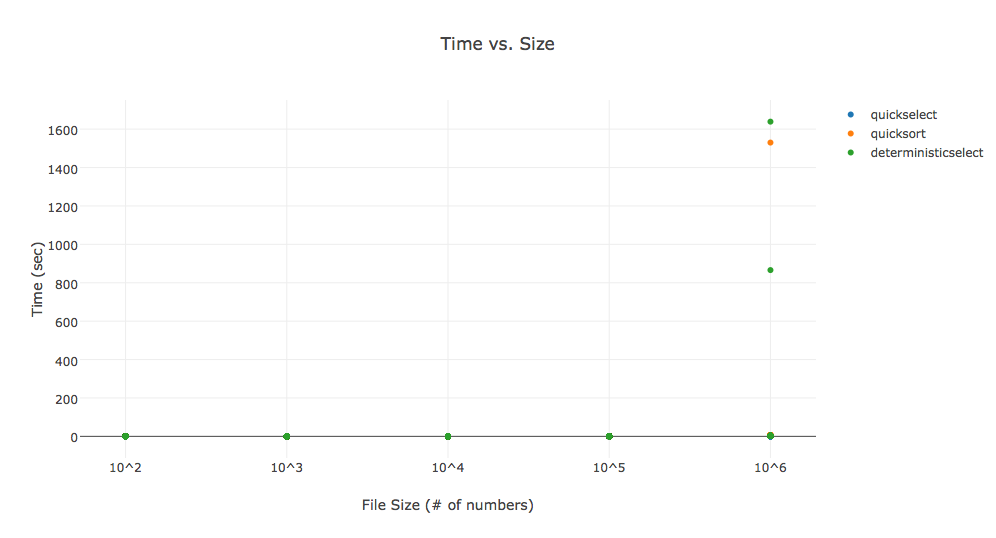
\includegraphics[scale=0.45]{resultsWoutliers}

Three outliers, two from deterministicselect and one from quicksort, clearly skewed our plot. We examined the lists that took substantially longer to complete to determine why - turns out Russell's computer had shifted into sleep mode and resumed executing once awoken. We felt justified in excluding the outliers and recreated the previous plot to gain a better sense of each algorithm's performance.

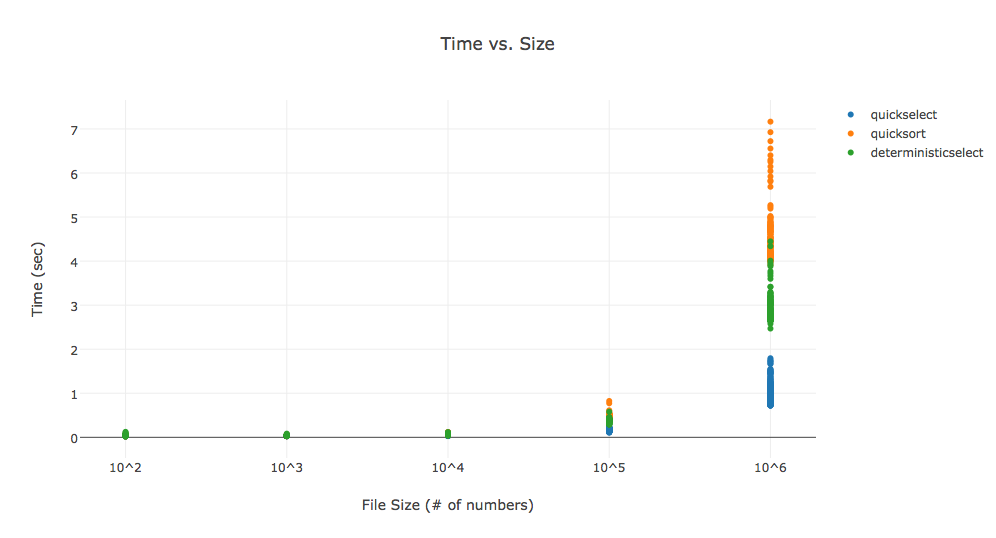
\includegraphics[scale=.45]{results}

To compare performance by list length, we plotted the performance of all three algorithms in a histogram for each of the five list lengths ($10^2, 10^3, 10^4, 10^5, 10^6$, respectively).

\section*{Conclusion}

\section*{Citations}
Quicksort. Wikipedia. Accessed June 6th, 2016. \url{https://en.wikipedia.org/wiki/Quicksort}\\

\noindent Quickselect. Wikipedia. Accessed June 6th, 2016. \url{https://en.wikipedia.org/wiki/Quickselect}\\

\noindent Median of Medians. Wikipedia. Accessed June 6th, 2016. \url{https://en.wikipedia.org/wiki/Median_of_medians}

\end{document}
